%%\textbf{}%%%%%%%%%%%%%%%%%%%%%%%%%%%%%%%%%%%%%%%%%%%%%%%%%%%%%%%%%%%%%%%%%%%%%%%%%%%%%%
%2345678901234567890123456789012345678901234567890123456789012345678901234567890
%        1         2         3         4         5         6         7         8
% THESIS CHAPTER


\chapter{Other Algorithms for Object Detection}
\label{chap:AppendixVision}
\ifpdf
    \graphicspath{{Vision/Figures/PNG/}{Vision/Figures/PDF/}{Vision/Figures/}}
\else
    \graphicspath{{Vision/Figures/EPS/}{Vision/Figures/}}
\fi

During the simulations, several trials have been done to find a suitable algorithm for the detection of the hole structure. In section (TODO) %todo ref sect
two methods have been discussed as the successful ones. In this appendix, others are briefly explained and discussed. Even if they are not used in the last versions of experiments, they can be useful for other purposes, such as detection of other kind of shapes. They can also be useful when the scene is different, for example while taking the hole structure from its side.\\
Each one is taken from \href{https://docs.opencv.org/3.4/d9/d97/tutorial_table_of_content_features2d.html}{OpenCV Detection tutorials}, where also other algorithms can be found.

\section{Corner Detection with the Shi-Harris method}

\begin{figure}[H]
	\centering
	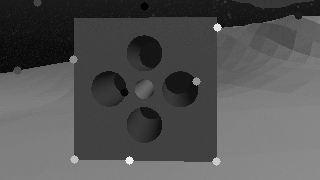
\includegraphics[width=8.0cm]{goodFeatToTrack}
	\caption[Result of \textit{goodFeaturesToTrack()}]{\textit{goodFeaturesToTrack()} result. Only two detected points are real corners, and the upper corners are not detected} 
	\label{fig:goodFeatToTrack}
\end{figure}


Following the \href{https://docs.opencv.org/3.4.6/d8/dd8/tutorial_good_features_to_track.html}{tutorial}, I implemented a corner detector with the Shi-Harris method [\cite{Shi94goodfeatures}] using the OpenCV function \href{https://docs.opencv.org/3.4.6/dd/d1a/group__imgproc__feature.html#ga1d6bb77486c8f92d79c8793ad995d541}{goodFeaturesToTrack()}.\\
This function acts as corner detector. In our case, this can be useful to find corners of the square hole structure. These points can be used successively as starting point to higher level vision algorithms (e.g. draw the square shape to then understand its pose).\\
The original example lets change the number of maximum points to be found. This is useful to reduce the number of false positive corners. The main problem is that the real corners of the square are not the "best" ones. So we can't simply put this parameter equal to 4. On the other side, with bigger number of points, is then difficult to discriminate the right corners from the others.\\
Other interesting parameters are:
\begin{itemize}
	\item \textbf{minDistance} The minimum distance between corners to be found.
	\item \textbf{qualityLevel} Parameter characterizing the minimal accepted quality of image corners.
	\item \textbf{blockSize} Size of an average block for computing a derivative covariation matrix over each pixel neighbourhood.
	\item \textbf{mask} To specify a certain region of interest in the image. In such a way, corners are found only in this region. The problem in our case is that without prior works we can't know where is the hole surface.
\end{itemize}
The points detected are effectively good feature points (as can be see in \ref{fig:goodFeatToTrack}). But the best ones, are not the ones that we want to detect (ie, the corner of the square).\\
This method should be used as a low level algorithm, to then help higher level ones. For example, to construct some polygons and to check if these polygons are square/rectangles. However, to follow this direction should be better to start from the edges. Another function can be to initialize a tracking by keypoints.\\
  
\section{Canny Edge and Hough Transform}
\label{sec:HoughTrasf}
%https://docs.opencv.org/3.4/d9/db0/tutorial_hough_lines.html

\begin{figure}[H]
	\centering
		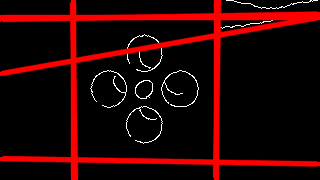
\includegraphics[width=5.0cm]{canny_HoughStandard}
		\qquad
		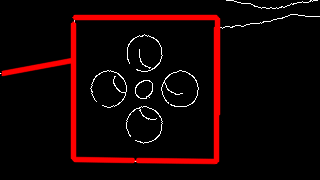
\includegraphics[width=5.0cm]{canny_HoughProb}
	\caption[Result of Standard Hough Transform and Probabilistic one]{Result of Hough Standard Transform (left) and Probabilistic (right). In white all the edges detected with Canny, in red the detected straight lines}
	\label{fig:HoughStandard}
\end{figure}

The Hough Transform [\cite{DudaHoughTrasf}] is a method to detect straight lines in an image. Usually, a preprocessing of the image with an edge detector is used to improve the results, for example with a Canny Edge Detector [\cite{CannyEdge}]. The OpenCV \href{https://docs.opencv.org/3.4/d9/db0/tutorial_hough_lines.html}{tutorial} makes use of two types of Hough Transform: the standard \href{https://docs.opencv.org/3.4/dd/d1a/group__imgproc__feature.html#ga46b4e588934f6c8dfd509cc6e0e4545a}{\textit{HoughLines()}} and the probabilistic \href{https://docs.opencv.org/3.4/dd/d1a/group__imgproc__feature.html#ga8618180a5948286384e3b7ca02f6feeb}{\textit{HoughLinesP()}} [\cite{houghprob}].\\
Results are visible in \ref{fig:HoughStandard}. The probabilistic method shows that this function is good to detect the square structure of the hole. 
Thus, this method can be used as good starting point to further process the image, to then estimate the pose of the hole, or of other objects of interest.

\section{Bounding Boxes Detection}
%https://docs.opencv.org/3.4.6/de/d62/tutorial_bounding_rotated_ellipses.html	

\begin{figure}[H]
	\centering
	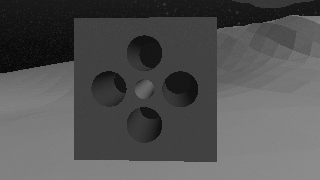
\includegraphics[width=5.0cm]{BoundBox_sourceOnlyPolig}
	\qquad
	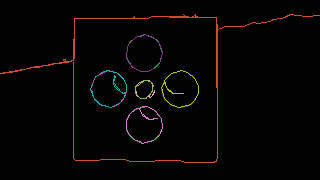
\includegraphics[width=5.0cm]{BoundBox_resultOnlyPolig}
	\caption[Result of bounding box detection]{Result of the algorithm: on the left the original image, on the right the contours detected}
	\label{fig:BoundBoxresultOnlyPolig}
\end{figure}

\begin{figure}[H]
	\centering
	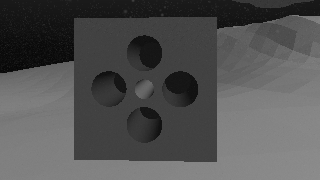
\includegraphics[width=5.0cm]{BoundBox_SourceOnlyRect}
	\qquad
	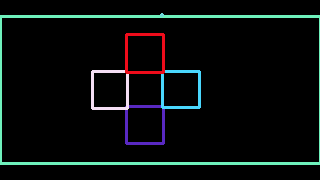
\includegraphics[width=5.0cm]{BoundBox_resultOnlyRect}
	\caption[Another result of bounding box detection]{On the left, the original image. On the right, the drawn bounding boxes around the holes.}
	\label{fig:BoundBoxresultOnlyRect}
\end{figure}

In this method, shape contours are found and then bounding boxes drawn. As explained in the previous section, finding shape contours can be a starting point to initialize higher level image processing, such as the tracking.\\
The code derived from an OpenCV \href{https://docs.opencv.org/3.4.6/de/d62/tutorial_bounding_rotated_ellipses.html}{tutorial}.\\
First, a Canny edge detector is used to preprocess the image. Then, the function \href{https://docs.opencv.org/3.4.6/d3/dc0/group__imgproc__shape.html#ga17ed9f5d79ae97bd4c7cf18403e1689a}{\textit{findContours()}} is called to retrieves contours with the algorithm described in \cite{findcountors}. Finally, rectangles are draw around as a bounding boxes.\\
In case of the square hole structure (already almost a "bounding box" of itself), finding the boxes is useful to reduce the noise, and to have a square/rectangle with straight lines.\\
The result without the bounding boxes are shown in \ref{fig:BoundBoxresultOnlyPolig}. The square is noticeable, but also other not interesting lines are shown. 
For this specific purpose (detection of square face of hole), the detection is worse than the algorithm of section \ref{sec:HoughTrasf} which used probabilistic hough transform.\\
The thing to notice is that the holes on the surface are well visible. This may be useful for other algorithms, or to detect other kind of shapes like a tube hole (a pipe).\\
Results in \ref{fig:BoundBoxresultOnlyRect} show bounding boxes around the holes. However, it is difficult to have a precise pose estimation with bounding boxes.\\
In conclusion, this is a good method that can be explored.
However, lot of non interesting edge are detected, so parameters have to be chosen wisely.


\section{2D Feature Matching \& Homography}
%https://docs.opencv.org/3.4/d7/dff/tutorial_feature_homography.html
\begin{figure}[H]
	\centering
	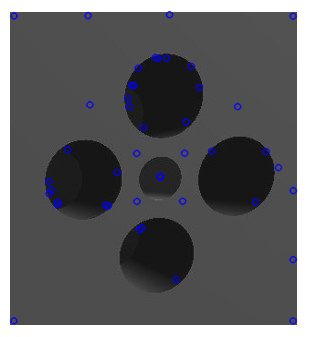
\includegraphics[width=3.8cm]{new_featHomog_SURF_templKeyPoint}\\
	\vspace{15px}
	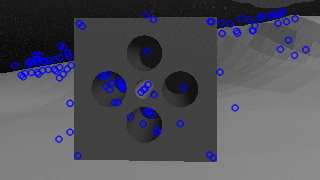
\includegraphics[width=6.2cm]{new_featHomog_SURF_cameraKeyPoint}
	\qquad
	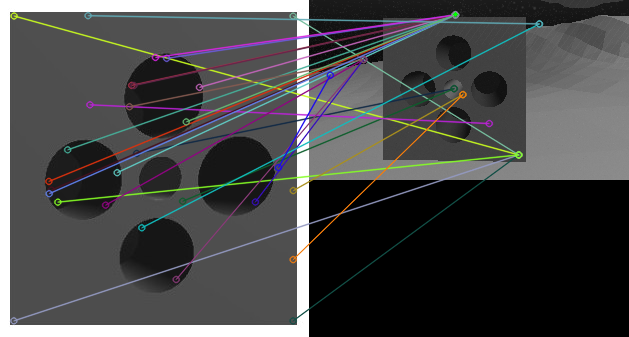
\includegraphics[width=7cm]{new_featHomog_SURF_result}
	\caption[Result of 2D Feature Matching]{Result of the algorithm. Above, the detected features (in blue) in the \textit{object image}. Below, on the left, the detected features in the \textit{scene image}; on the right the matched (erroneous) features.}
	\label{fig:featHomog}
\end{figure}

\textit{Image features} are small patches that are useful to compute similarities between images. Please note that these features are different from corner points.
They indicates particular details that are different from others. Detecting these areas is important to recognize objects of interest in the image. The \textit{descriptors} of these features contain the visual description of the patches, and they are used to recognize similarities.\\
This method uses a \textit{object image} and a \textit{scene image}. The first is a sort of template (note that this method is not a template matching (TODO CITA MY SEZ)) %todo cita sezione template match?)
which contains only the object to be found (in this case, the square face of the hole). The second is the image in which we want to detect this object (in this case, what the camera is seeing).\\
After good \textit{features} are extracted from both images, the \textit{descriptors} are used to match them, thus, detecting the object in the scene.
Then, it is necessary to find the perspective transformation between object image and the scene (i.e. find homography). This is needed to take into account that usually pose and scaling of the object in the scene are not the same of the object image.\\
The OpenCV \href{https://docs.opencv.org/3.4/d7/dff/tutorial_feature_homography.html}{tutorial} use different tools:
\begin{itemize}
	\item \textbf{SURF} (Speeded Up Robust Features) Detector [\cite{surfDet}] to extract features from \textit{object image} and \textit{scene image}, and to compute descriptors.
	\item \textbf{FLANN} (Fast Library for Approximate Nearest Neighbors) matcher [\cite{flannMatch}] to match the features.
	\item \textbf{Lowe's ratio test} [\cite{loweTest}]to filter the best matches.
	\item \textbf{RANSAC} (RANdom SAmple Consensus) [\cite{ransacHomog}] method to find the homography with the function \href{https://docs.opencv.org/3.4/d9/d0c/group__calib3d.html#ga4abc2ece9fab9398f2e560d53c8c9780}{\textit{findHomography()}}.
\end{itemize}

In this case, results are unsatisfactory as can be seen in \ref{fig:featHomog}. The main problem is that in this particular scene there are not nice distinct features. Also, the symmetry of the structure does not help, because there are a lot of particulars that are the same (like the square side and the holes). As can be seen in the \href{https://docs.opencv.org/3.4/d7/dff/tutorial_feature_homography.html}{tutorial}, good results are obtained for food boxes. In fact, this methods is often associate to scenes where a lot of details are present (graffiti painting, supermarket shelf, ...). In our underwater case, realistic infrastructures don't have this details.\\
There are also lot of parameters to set for the three main tools (SURF, FLANN, RANSAC). Various trials have been tried but no-one was satisfactory. Also, different detectors (like SWIFT [\cite{loweTest}]) and matchers (like Brute-force), have been tried.\\
The variety of tools and parameters make this method suitable for a lot of applications, and must be taken into consideration in other applications.







